\documentclass{article}

\title{When Rust hurts}
\subtitle{Why I am not enjoying programming in Rust.}
\reddit{https://www.reddit.com/r/rust/comments/112hmga/blog_post_when_rust_hurts/}
\hackernews{https://news.ycombinator.com/item?id=34803379}
\date{2023-02-14}
\modified{2023-02-16}

\keyword{rust}

\begin{document}
\epigraph{
  Functional programming deals with values; imperative programming deals with objects.
}{Alexander Stepanov, ``Elements of Programming'', p. 5}

\section{intro}{Introduction}

\href{https://www.rust-lang.org/}{Rust} is in a sweet spot in the language design space.
It allows us to build efficient and memory-safe programs with concise, portable, and sometimes even pretty code.

However, it is not all roses and sunshine.
Memory management details often stay in your way and make the code uglier or more repetitive than it could be in a ``higher-level'' programming language, such as \href{https://www.haskell.org/}{Haskell} or \href{https://ocaml.org}{OCaml}.
In almost all cases, these issues are not defects of the compiler but direct consequences of the Rust's team design choices.

This article details on how frustrating Rust can be if you approach it with a functional programming mindset and why Rust has no choice but to frustrate you.

\section{objects-values-references}{Objects, values, and references}
\epigraph{
    Values and objects play complementary roles.
    Values are unchanging and independent of any particular implementation in the computer.
    Objects are changeable and have computer-specific implementations.
}{Alexander Stepanov, ``Elements of Programming'', p. 5}

Understanding the difference between objects, values, and references is helpful before diving deeper into Rust.

In the context of this article, \emph{values} are entities with distinct identities, such as numbers and strings.
An \emph{object} is a representation of a value in the computer memory.
A \emph{reference} is the address of an object that we can use to access the object or its parts.

\begin{figure}[grayscale-diagram]
\marginnote{mn-objects-values-refs}{
  A visualization of values, objects, and references on an example of an integer in a 16-bit computer.
  The value is number five, which has no inherent type.
  The object is a 16-bit integer stored at address \code{0x0300} (\href{https://en.wikipedia.org/wiki/Endianness}{little-endian}).
  The memory contains a \emph{reference} to the number, represented as a pointer to address \code{0x0300}.
}
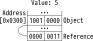
\includegraphics{/images/15-objects-values-references.svg}
\end{figure}

System programming languages, such as C++ and Rust, force the programmer to deal with the distinction between objects and references.
This distinction allows us to write blazingly fast code, but it comes with a high price: it is a never-ending source of bugs.
It is almost always a bug to modify the contents of an object if some other part of the program references that object.
There are multiple ways to address this issue:

\begin{itemize}
  \item
    Ignore the problem and trust the programmer.
    Most traditional system programming languages, such as C++, took this path.
  \item
    Make all objects immutable.
    This option is the basis for pure functional programming techniques in Haskell and \href{https://clojure.org/}{Clojure}.
  \item
    Adopt a \href{https://en.wikipedia.org/wiki/Substructural_type_system}{type system} preventing modification of referenced objects.
    Languages such as \href{https://www.cs.bu.edu/~hwxi/atslangweb/}{ATS} and Rust embarked on this journey.
  \item
    Ban references altogether.
    The \href{https://www.val-lang.dev/}{Val} language explores this style of programming.
\end{itemize}

The distinction between objects and references is also a source of accidental complexity and choice explosion.
A language with immutable objects and automatic memory management allows us to stay ignorant of this distinction and treat everything as a value (at least in pure code).
A unified storage model frees up a programmer's mental resources and enables her to write more expressive and elegant code.
However, what we gain in convenience, we lose in efficiency: pure functional programs often require more memory, can become unresponsive, and are harder to optimize (your mileage may vary).

\section{abstraction-hurts}{When abstraction hurts}

Manual memory management and the ownership-aware type system interfere with our ability to break down the code into smaller pieces.

\subsection{common-expression-elimination}{Common expression elimination}

Extracting a common expression into a variable can pose unexpected challenges.
Let us start with the following snippet of code.

\begin{code}[rust]
let x = f("a very long string".to_string());
let y = g("a very long string".to_string());
// \ldots
\end{code}

Look, \code{"a very long string".to_string()} appears twice!
Our first instinct is to assign a name to the expression and use it twice:

\begin{code}[good]
let \b{s} = "a very long string".to_string();
let x = f(\b{s});
let y = g(\b{s});
\end{code}

However, our first naive version will not compile because the \code{String} type does not implement the \code{Copy} trait.
We must write the following expression instead:

\begin{code}[good]
let s = "a very long string".to_string();
f(s\b{.clone()});
g(s);
\end{code}

We can see the extra verbosity in a positive light if we care about extra memory allocations because copying memory became explicit.
But it can be quite annoying in practice, especially when you add \code{h(s)} two months later.

\begin{code}[bad]
let s = "a very long string".to_string();
f(s.clone());
g(s);

// fifty lines of code...

h(s); // ← won't compile, you need scroll up and update g(s).
\end{code}

\subsection{monomorphism-restriction}{Monomorphism restriction}

In Rust, \code{let x = y;} does not always mean that \code{x} is the same thing as \code{y}.
One example of when this natural property breaks is when \code{y} is an overloaded function.

For example, let us define a short name for an overloaded function.

\begin{code}[bad]
// Do we have to type "MyType::from" every time?
// How about introducing an alias?
let x = MyType::from(b"bytes");
let y = MyType::from("string");

// Nope, Rust won't let us.
let f = MyType::from;
let x = f(b"bytes");
let y = f("string");
//      - ^^^^^^^^ expected slice `[u8]`, found `str`
//      |
//      arguments to this function are incorrect
\end{code}

The snippet does not compile because the compiler will bind \code{f} to a particular instance of \code{MyType::from}, not to a polymorphic function.
We have to make \code{f} polymorphic explicitly.

\begin{code}[good]
// Compiles fine, but is longer than the original.
fn f<T: Into<MyType>>(t: T) -> MyType { t.into() }

let x = f(b"bytes");
let y = f("string");
\end{code}

Haskell programmers might find this problem familiar: it looks suspiciously similar to the dreaded \href{https://wiki.haskell.org/Monomorphism_restriction}{monomorphism restriction}!
Unfortunately, \code{rustc} does not have the \href{https://typeclasses.com/ghc/no-monomorphism-restriction}{\code{NoMonomorphismRestriction}} pragma.

\subsection{functional-abstraction}{Functional abstraction}

Factoring code into a function might be harder than you expect because the compiler cannot reason about aliasing across function boundaries.
Let's say we have the following code.

\begin{code}[rust]
impl State {
  fn tick(&mut self) {
    self.state = match self.state {
      Ping(s) => { self.x += 1; Pong(s) }
      Pong(s) => { self.x += 1; Ping(s) }
    }
  }
}
\end{code}

The \code{self.x += 1} statement appears multiple times.
Why not extract it into a method\ldots

\begin{code}[bad]
impl State {
  fn tick(&mut self) {
    self.state = match self.state {
      Ping(s) => { self.inc(); Pong(s) } // ← compile error
      Pong(s) => { self.inc(); Ping(s) } // ← compile error
    }
  }

  fn inc(&mut self) {
    self.x += 1;
  }
}
\end{code}

Rust will bark at us because the method attempts to re-borrow \code{self} exclusively while the surrounding context still holds a mutable reference to \code{self.state}.

Rust 2021 edition implemented \href{https://doc.rust-lang.org/edition-guide/rust-2021/disjoint-capture-in-closures.html}{disjoint capture} to address a similar issue with closures.
Before Rust 2021, code that looked like \code{x.f.m(|| x.y)} might not compile but manually inlining \code{m} and the closure would resolve the error.
For example, imagine we have a struct that owns a map and a default value for map entries.

\begin{code}[bad]
struct S { map: HashMap<i64, String>, def: String }

impl S {
  fn ensure_has_entry(&mut self, key: i64) {
    // Doesn't compile with Rust 2018:
    self.map.entry(key).or_insert_with(|| self.def.clone());
// |         ------            -------------- ^^ ---- second borrow occurs...
// |         |                 |              |
// |         |                 |              immutable borrow occurs here
// |         |                 mutable borrow later used by call
// |         mutable borrow occurs here
  }
}
\end{code}

However, if we inline the definition of \code{or_insert_with} and the lambda function, the compiler can finally see that the borrowing rules hold.

\begin{code}[good]
struct S { map: HashMap<i64, String>, def: String }

impl S {
  fn ensure_has_entry(&mut self, key: i64) {
    use std::collections::hash_map::Entry::*;
    \emph{// This version is more verbose, but it works with Rust 2018.}
    match self.map.entry(key) {
      Occupied(mut e) => e.get_mut(),
      Vacant(mut e) => e.insert(self.def.clone()),
    };
  }
}
\end{code}

When someone asks you, ``what tricks can Rust closures do that named functions cannot?'' you will know the answer: they can capture only the fields they use.

\subsection{newtype-abstrction}{Newtype abstraction}

The \href{https://doc.rust-lang.org/rust-by-example/generics/new_types.html}{new type idiom}\sidenote{sn-strong-typedef}{
  Folks in the C++ land call this idiom \href{https://www.boost.org/doc/libs/1_42_0/boost/strong_typedef.hpp}{strong typedef}.
} in Rust allows the programmer to give a new identity to an existing type.
The idiom's name comes from Haskell's \href{https://wiki.haskell.org/Newtype}{\code{newtype}} keyword.

One of the common uses of this idiom is to work around the \href{#orphan-rules}{orphan rules} and define trait implementation for the aliased type.
For example, the following code defines a new type that displays byte vectors in hex.

\begin{code}[rust]
struct Hex(Vec<u8>);

impl std::fmt::Display for Hex {
  fn fmt(&self, f: &mut std::fmt::Formatter<'_>) -> std::fmt::Result {
    self.0.iter().try_for_each(|b| write!(f, "{:02x}", b))
  }
}

println!("{}", Hex((0..32).collect()));
\emph{// => 000102030405060708090a0b0c0d0e0f101112131415161718191a1b1c1d1e1f}
\end{code}

The new type idiom is efficient: the representation of the \code{Hex} type in the machine's memory is identical to that of \code{Vec<u8>}.
However, despite the identical representation, the compiler does not treat our new type as a strong alias for \code{Vec<u8>}.
For example, we cannot safely transform \code{Vec<Hex>} to \code{Vec<Vec<u8>>} and back without reallocating the outer vector.
Also, without copying the bytes, we cannot safely coerce \code{\&Vec<u8>} to \code{\&Hex}.

\begin{code}[rust]
fn complex_function(bytes: &Vec<u8>) {
  // \ldots  a lot of code \ldots

  println!("{}", &Hex(bytes));        // That does not work.
  println!("{}", Hex(bytes.clone())); // That works but is slow.

  // \ldots  a lot of code \ldots
}
\end{code}

Overall, the newtype idiom is a leaky abstraction because it is a convention, not a first-class language feature.
If you wonder how Haskell solved this problem, I recommend watching the \href{https://www.youtube.com/watch?v=iLZdN-R1JGk}{Safe, Zero-Cost Coercions in Haskell} talk by Simon Peyton Jones.

\subsection{views-and-bundles}{Views and bundles}

Each time the programmer describes a struct field or passes an argument to a function, she must decide whether the field/argument should be \href{#objects-values-references}{an object or a reference}.
Or maybe the best option is to \href{https://doc.rust-lang.org/std/borrow/enum.Cow.html}{decide at runtime}?
That is a lot of decision-making!
Unfortunately, sometimes there is no optimal choice.
On such occasions, we grit our teeth and define several versions of the same type with slightly different field types.

Most functions in Rust take arguments by reference and return results as a self-contained object\sidenote{sn-view-exceptions}{
  There are plenty of exceptions, of course.
  Sometimes we pass arguments by value if making a copy is cheap or the function can efficiently reuse its input to produce the result.
  Some functions return references to one of their arguments.
}.
This pattern is so common that it might be helpful to define new terms.
I call input types with lifetime parameters \emph{views} because they are optimal for inspecting data.
I call regular output types \emph{bundles} because they are self-contained.

The following snippet comes from the (sunset) \href{https://github.com/bytecodealliance/lucet}{Lucet} WebAssembly runtime.
\begin{code}[rust]
\emph{/// A WebAssembly global along with its export specification.}
\emph{/// The lifetime parameter exists to support zero-copy deserialization}
\emph{/// for the `\&str` fields at the leaves of the structure.}
\emph{/// For a variant with owned types at the leaves, see `OwnedGlobalSpec`.}
pub struct \href{https://github.com/bytecodealliance/lucet/blob/51fb1ed414fe44f842db437d94abb6eb439d7c92/lucet-module/src/globals.rs#L8}{\code{GlobalSpec}}<'a> {
    global: Global<'a>,
    export_names: Vec<&'a str>,
}

\ldots

\emph{/// A variant of `GlobalSpec` with owned strings throughout.}
\emph{/// This type is useful when directly building up a value to be serialized.}
pub struct \href{https://github.com/bytecodealliance/lucet/blob/51fb1ed414fe44f842db437d94abb6eb439d7c92/lucet-module/src/globals.rs#L112}{\code{OwnedGlobalSpec}} {
    global: OwnedGlobal,
    export_names: Vec<String>,
}
\end{code}

The authors duplicated the \code{GlobalSpec} data structure to support two use cases:
\begin{itemize}
  \item
    \code{GlobalSpec<'a>} is a \emph{view} object that the code authors parse from a byte buffer.
    Individual fields of this view point back to the relevant regions of the buffer.
    This representation is helpful for functions that need to inspect values of type \code{GlobalSpec} without modifying them.
  \item
    \code{OwnedGlobalSpec} is a \emph{bundle}: it does not contain references to other data structures.
    This representation is helpful for functions that construct values of type \code{GlobalSpec} and pass them around or put them into a container.
\end{itemize}

In a language with automatic memory management, we can combine the efficiency of \code{GlobalSpec<'a>} with the versatility of \code{OwnedGlobalSpec} in a single type declaration.

\section{composition-hurts}{When composition hurts}

Building a working program from smaller pieces can be frustrating in Rust.

\subsection{object-composition}{Object composition}

When programmers have two distinct objects, they often want to combine them into a single structure.
Sounds easy? Not in Rust.

Assume we have an object \code{Db} that has a method giving you another object, \code{Snapshot<'a>}.
The lifetime of the snapshot depends on the lifetime of the database.

\begin{code}[rust]
struct Db { /* \ldots  */ }

struct Snapshot<'a> { /* \ldots  */ }

impl Db { fn snapshot<'a>(&'a self) -> Snapshot<'a>; }
\end{code}

We might want to bundle\sidenote{sn-db-iterator}{
  If you wonder why we have this strange desire, you can read comments from the \href{https://sourcegraph.com/github.com/dfinity/ic@d14361f9939baaeb899106b874851ad4a0ce928b/-/blob/rs/artifact_pool/src/rocksdb_iterator.rs?L153-164}{\code{rocksdb_iterator.rs}} module.
} the database with its snapshot, but Rust will not let us.

\begin{code}[bad]
\emph{// There is no way to define the following struct without}
\emph{// contaminating it with lifetimes.}
struct DbSnapshot {
  snapshot: Snapshot<'a>, \emph{// what should 'a be?}
  db: Arc<Db>,
}
\end{code}

Rust folks call this arrangement ``sibling pointers''.
Rust forbids sibling pointers in safe code because they undermine Rust's safety model.

As discussed in the \href{#objects-values-references}{Objects, values, and references} section, modifying a referenced object is usually a bug.
In our case, the \code{snapshot} object might depend on the physical location of the \code{db} object.
If we move the \code{DbSnapshot} as a whole, the physical location of the \code{db} field will change, corrupting references in the \code{snapshot} object.
We \emph{know} that moving \code{Arc<Db>} will not change the location of the \code{Db} object, but there is no way to communicate this information to \code{rustc}.

Another issue with \code{DbSnapshot} is that the order of its field \href{https://doc.rust-lang.org/stable/reference/destructors.html}{destruction} matters.
If Rust allowed sibling pointers, changing the field order could introduce undefined behavior: the \code{snapshot}'s destructor could try to access fields of a destroyed \code{db} object.

\subsection{pattern-matching-boxes}{Pattern matching cannot see through boxes}

In Rust, we cannot pattern-match on boxed types such as \code{Box}, \code{Arc}, \code{String}, and \code{Vec}.
This restriction is often a deal-breaker because we cannot avoid boxing when we define recursive data types.

For example, let us try to match a vector of strings.

\begin{code}[bad]
let x = vec!["a".to_string(), "b".to_string()];
match x {
//    - help: consider slicing here: `x[..]`
    ["a", "b"] => println!("OK"),
//  ^^^^^^^^^^ pattern cannot match with input type `Vec<String>`
    _ => (),
}
\end{code}

First, we can't match a vector, only on a slice.
Luckily, the compiler suggests an easy fix: we must replace \code{x} with \code{x[..]} in the \code{match} expression.
Let us give it a try.

\begin{code}[bad]
let x = vec!["a".to_string(), "b".to_string()];
match x[..] {
//    ----- this expression has type `[String]`
    ["a", "b"] => println!("OK"),
//   ^^^ expected struct `String`, found `&str`
    _ => (),
}
\end{code}

As you can see, removing one layer of boxes is not enough to make the compiler happy.
We also need to unbox the strings inside of the vector, which is not possible without allocating a new vector:

\begin{code}[good]
let x = vec!["a".to_string(), "b".to_string()];
// We have to allocate new storage.
let x_for_match: Vec<_> = x.iter().map(|s| s.as_str()).collect();
match &x_for_match[..] {
    ["a", "b"] => println!("OK"), // this compiles
    _ => (),
}
\end{code}

Forget about \href{https://www.cs.tufts.edu/comp/150FP/archive/chris-okasaki/redblack99.pdf}{balancing Red-Black trees} in five lines of code in Rust.

\subsection{orphan-rules}{Orphan rules}

Rust uses \href{https://doc.rust-lang.org/reference/items/implementations.html?highlight=orphan#orphan-rules}{orphan rules} to decide whether a type can implement a trait.
For non-generic types, these rules forbid implementing a trait for a type outside of crates defining the trait or the type.
In other words, the package defining the trait must depend on the package defining the type or vice versa.

\begin{figure}[grayscale-diagram]
\marginnote{mn-orphan-rules}{
  Orphan rules in Rust demand that a trait implementation resides in the crate defining the trait or the crate defining the type.
  Boxes represent separate crates, arrows---crate dependencies.
}
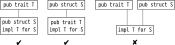
\includegraphics{/images/15-orphan-rules.svg}
\end{figure}

These rules make it easy for the compiler to guarantee \emph{coherence}, which is a smart way to say that all parts of your program see the same trait implementation for a particular type.
In exchange, this rule significantly complicates integrating traits and types from unrelated libraries.

One example is traits we want to use only in tests, such as \href{https://altsysrq.github.io/rustdoc/proptest/1.0.0/proptest/arbitrary/trait.Arbitrary.html}{\code{Arbitrary}} from the \href{https://crates.io/crates/proptest}{proptest} package.
We can save a lot of typing if the compiler derives implementations for types from our package, but we want our production code to be independent of the \code{proptest} package.
In the perfect setup, all the \code{Arbitrary} implementations would go into a separate test-only package.
Unfortunately, orphan rules oppose this arrangement, forcing us to bite the bullet and write proptest strategies \href{https://altsysrq.github.io/proptest-book/proptest/tutorial/macro-prop-compose.html}{manually} instead\sidenote{sn-orphan-workaround}{
  There are workarounds for this issue, such as using \href{https://doc.rust-lang.org/cargo/reference/features.html}{cargo features} and conditional compilation, but they complicate the build setup so much that writing boilerplate is usually a better option.
}.


Type conversion traits, such as \code{From} and \code{Into}, are also problematic under orphan rules.
I often see \code{xxx-types} packages that start small but end up as bottlenecks in the compilation chain.
Splitting such packages into smaller pieces is often daunting because of the intricate webs of type conversions connecting distant types together.
Orphan rules do not allow us to cut these packages on module boundaries and move all conversions into a separate package without doing a lot of tedious work.

Do not get me wrong: orphan rules are a great default.
Haskell allows you to define \href{https://wiki.haskell.org/Orphan_instance}{orphan instances}, but programmers frown upon this practice.
It is the inability to escape orphan rules that makes me sad.
In large codebases, decomposing large packages into smaller pieces and maintaining shallow dependencies graphs are the only path to acceptable compilation speed.
Orphan rules often stay in the way of trimming dependency graphs.

\section{fearless-concurrency}{Fearless concurrency is a lie}

The Rust team coined the term \href{https://blog.rust-lang.org/2015/04/10/Fearless-Concurrency.html}{Fearless Concurrency} to indicate that Rust helps you avoid common pitfalls associated with parallel and concurrent programming.
Despite these claims, my \href{https://en.wikipedia.org/wiki/Cortisol}{cortisol} level goes up every time I introduce concurrency to my Rust programs.

\subsection{deadlocks}{Deadlocks}
\epigraph{
    So it's perfectly ``fine'' for a Safe Rust program to get deadlocked or do something nonsensical with incorrect synchronization.
    Obviously such a program isn't very good, but Rust can only hold your hand so far.
}{The Rustonomicon, \href{https://doc.rust-lang.org/nomicon/races.html}{Data Races and Race Conditions}}

Safe Rust prevents a specific type of concurrency bug called \emph{data race}.
Concurrent Rust programs have plenty of other ways to behave incorrectly.

One class of concurrency bugs that I experienced firsthand is \href{https://en.wikipedia.org/wiki/Deadlock}{deadlock}.
A typical explanation of this class of bugs involves two locks and two processes trying to acquire the locks in opposite orders.
However, if the locks you use are not \href{https://stackoverflow.com/questions/1312259/what-is-the-re-entrant-lock-and-concept-in-general}{re-entrant} (and Rust's locks are not), having a single lock is enough to cause a deadlock.

For example, the following code is buggy because it attempts to acquire the same lock twice.
The bug might be hard to spot if \code{do_something} and \code{helper_function} are large and live far apart in the source file or if we call \code{helper_function} on a rare execution path.

\begin{code}[bad]
impl Service {
  pub fn do_something(&self) {
    let guard = self.lock.read();
    \emph{// \ldots }
    self.helper_function(); \emph{// \b{BUG}: will panic or deadlock}
    \emph{// \ldots }
  }

  fn helper_function(&self) {
    let guard = self.lock.read();
    \emph{// \ldots }
  }
}
\end{code}

The documentation for \href{https://doc.rust-lang.org/std/sync/struct.RwLock.html#method.read}{\code{RwLock::read}} mentions that the function \emph{might} panic if the current thread already holds the lock.
All I got was a hanging program.

Some languages tried to provide a solution to this problem in their concurrency toolkits.
The Clang compiler has \href{https://clang.llvm.org/docs/ThreadSafetyAnalysis.html}{Thread safety annotations} enabling a form of static analysis that can detect race conditions and deadlocks.
However, the best way to avoid deadlocks is not to have locks.
Two technologies that approach the problem fundamentally are \href{https://en.wikipedia.org/wiki/Software_transactional_memory}{Software Transaction Memory} (implemented in \href{https://wiki.haskell.org/Software_transactional_memory}{Haskell}, \href{https://clojure.org/reference/refs}{Clojure}, and \href{https://nbronson.github.io/scala-stm/}{Scala}) and the \href{https://en.wikipedia.org/wiki/Actor_model}{actor model} (\href{https://www.erlang.org/}{Erlang} was the first language that fully embraced it).

\subsection{filesystem-shared-resource}{Filesystem is a shared resource}
\epigraph{
    We can view a path as an \emph{address}.
    Then a string representing a path is a pointer, and accessing a file through a path is a pointer dereference.
    Thus, component interference due to file overwriting can be viewed as an address collision problem: two components occupy overlapping parts of the address space.
}{Eelco Dolstra, \href{https://edolstra.github.io/pubs/phd-thesis.pdf}{The Purely Functional Software Deployment Model}, p. 53}

Rust gives us powerful tools to deal with shared memory.
However, once our programs need to interact with the outside world (e.g., use a network interface or a filesystem), we are on our own.
Rust is similar to most modern languages in this regard.
However, it can give you a false sense of security.

Remember that paths are raw pointers, even in Rust.
Most file operations are inherently unsafe and can lead to data races (in a broad sense) if you do not correctly synchronize file access.
For example, as of February 2023, I still experience a six-year-old \href{https://github.com/rust-lang/rustup/issues/988}{concurrency bug} in \href{https://rustup.rs/}{rustup}.

\subsection{implicit-async-runtimes}{Implicit async runtimes}
\epigraph{
    I cannot seriously believe in it because the theory cannot be reconciled with the idea that physics should represent a reality in time and space, free from spooky action at a distance.
}{Albert Einstein, \href{https://books.google.ch/books?redir_esc=y&hl=de&id=HvZAAQAAIAAJ&focus=searchwithinvolume&q=spooky+action}{The Born-Einstein letters}, p. 158.}

The value of Rust that I like the most is its focus on local reasoning.
Looking at the function's type signature often gives you a solid understanding of what the function can do.
State mutations are explicit thanks to mutability and lifetime annotations.
Error handling is explicit and intuitive thanks to the ubiquitous \code{Result} type.
When used correctly, these features often lead to the mystical \href{https://wiki.haskell.org/Why_Haskell_just_works}{if it compiles---it works} effect.
Asynchronous programming in Rust is different, however.

Rust supports the \href{https://rust-lang.github.io/async-book/01_getting_started/04_async_await_primer.html}{\code{async/.await}} syntax for defining and composing asynchronous functions, but the runtime support is limited.
Several libraries (called \href{https://ncameron.org/blog/what-is-an-async-runtime/}{async runtimes}) define asynchronous functions to interact with the operating system.
The \href{https://crates.io/crates/tokio}{tokio} package is the most popular library.

One common issue with runtimes is that they rely on passing arguments implicitly.
For example, the tokio runtime allows you to \href{https://docs.rs/tokio/latest/tokio/fn.spawn.html}{\code{spawn}} a concurrent task at any point in your program.
For this function to work, the programmer has to construct a runtime object in advance.

\begin{code}[rust]
fn innocently_looking_function() {
  \href{https://docs.rs/tokio/1.25.0/tokio/fn.spawn.html}{\code{tokio::spawn}}(some_async_func());
  // ^
  // |
  // \emph{This code will panic if we remove this line. Spukhafte Fernwirkung!}
} //                                     |
  //                                     |
fn main() { //                           v
  let _rt = \href{https://docs.rs/tokio/1.25.0/tokio/runtime/struct.Runtime.html}{\code{tokio::runtime::Runtime}}::new().unwrap();
  innocently_looking_function();
}
\end{code}

These implicit arguments turn compile-time errors into runtime errors.
What should have been a compile error turns into a debugging adventure:

\begin{itemize}
  \item
    If the runtime were an explicit argument, the code would not compile unless the programmer constructed a runtime and passed it as an argument.
    When the runtime is implicit, your code might compile fine but will crash at runtime if you forget to annotate your main function with a \href{https://docs.rs/tokio/latest/tokio/attr.main.html}{magical macro}.
  \item
    Mixing libraries that chose different runtimes is \href{https://www.ncameron.org/blog/portable-and-interoperable-async-rust/}{complicated}.
    The problem is even more confusing if it involves multiple major versions of the same runtime.
    My experience writing async Rust code resonates with the \href{https://rust-lang.github.io/wg-async/vision/submitted_stories/status_quo.html}{Status Quo} stories collected by the \href{https://rust-lang.github.io/wg-async/welcome.html}{Async Working Group}.
\end{itemize}

Some might argue that threading ubiquitous arguments through the entire call stack is unergonomic.
\href{/posts/03-rust-packages-crates-modules.html#explicit-dependencies}{Explicitly passing all arguments} is the only approach that scales well.

\subsection{functions-have-colors}{Functions have colors}
\epigraph{
    At this point, a reasonable person might think the language hates us.
}{Bob Nystrom, \href{https://journal.stuffwithstuff.com/2015/02/01/what-color-is-your-function/}{What Color is Your Function?}}

Rust's \code{async/.await} syntax simplifies the composition of asynchronous algorithms.
In return, it brings a fair amount of complexity, \href{https://journal.stuffwithstuff.com/2015/02/01/what-color-is-your-function/}{painting every function} in \emph{blue} (sync) or \emph{red} (async) color.
There are new rules to follow:
\begin{itemize}
  \item
    Sync functions can call other sync functions and get a result.
    Async functions can call and \code{.await} other async functions to get a result.
  \item
    We cannot directly call and await async functions from sync functions.
    We need an \href{#implicit-async-runtimes}{async runtime} that will execute an async function for us.
  \item
    We can call sync functions from async functions.
    But beware!
    Not all sync functions are equally blue.
\end{itemize}

That is it; some sync functions are secretly \emph{purple}: they can read files, join threads, or \href{https://doc.rust-lang.org/std/thread/fn.sleep.html}{\code{thread::sleep}} on a couch.
We do not want to call these purple (blocking) functions from red (async) functions because they will block the runtime and kill the performance benefits that motivated us to step into this asynchrony mess.

Unfortunately, purple functions are secretive: you cannot tell whether a function is purple without inspecting its body and the bodies of all other functions in its \href{https://en.wikipedia.org/wiki/Call_graph}{call graph}.
These bodies evolve, so we better keep an eye on them.

The real fun comes when you have a code base with shared ownership where multiple teams sandwich sync and async code.
Such packages tend to be bug silos, waiting for enough system load to manifest another purple defect in the sandwich that makes the system unresponsive.

Languages with runtimes built around \href{https://en.wikipedia.org/wiki/Green_thread}{green threads}, such as \href{https://haskell.org/}{Haskell} and \href{https://go.dev/}{Go}, eliminate the proliferation of function colors.
Building a concurrent program from independent components is easier and safer in such languages.

\section{conclusion}{Conclusion}
\epigraph{
    There are only two kinds of languages: the ones people complain about and the ones nobody uses.
}{\href{https://www.stroustrup.com/quotes.html}{Bjarne Stroustrup}}

Rust is a disciplined language that got many important decisions right, such as an uncompromising focus on safety, the trait system design\sidenote{sn-trait-system-cpp}{I'm looking at you, \href{https://en.cppreference.com/w/cpp/language/constraints}{C++ Concepts}.}, the lack of implicit conversions, and a holistic approach to \href{/posts/12-rust-error-handling.html}{error handling}.
It allows us to develop robust and memory-safe programs relatively quickly without compromising execution speed.

Yet, I often find myself overwhelmed with accidental complexity, especially when I care little about performance and want to get something working quickly (for example, in test code).
Rust can complicate \href{#abstraction-hurts}{decomposing} your program into smaller pieces and \href{#composition-hurts}{composing} it from smaller pieces.
Rust only partially eliminates the \href{#fearless-concurrency}{concurrency issues}.
Oh well, no language is perfect for every problem.

You can discuss this article on \href{https://www.reddit.com/r/rust/comments/112hmga/blog_post_when_rust_hurts/}{Reddit}.
\end{document}
